\documentclass[twocolumn]{article}
\hbadness=10000

% ====== Packages ======
\usepackage[utf8]{inputenc}       % Encoding
\usepackage{amsmath, amssymb}     % Math
\usepackage{graphicx}             % Images
\usepackage{hyperref}             % Hyperlinks
\usepackage{geometry}             % Page layout
\geometry{margin=0.3in}
\usepackage{subcaption}
\usepackage{parskip}

% ====== Metadata ======
\title{My Document Title}
\author{Your Name}
\date{\today}

% ====== Begin Document ======
\begin{document}

\maketitle

\begin{abstract}
This is a short summary of the document. You can describe the goals or the structure here.
\end{abstract}

\section{Introduction}
This is intended as a brainstorming documentation for the project

\section{Prior Works}
The existing studies have focused extensively on subsea cable inference methods,
meaning that each research would have adopted a set of primary assumptions,
and attempt to iteratively select information most closely aligned with the assumptions

Out of Sight, Not Out of Mind
\begin{enumerate}
    \item if there is no drivable routes between each ends of a given data path, there must not be a countinuous landmass connecting them
    \item Speed-of-light (SoL) constraints on hop RTT
    \item IP addresses associated with subsea cables can reveal information related to the cable owners
    \item RIPE Atlas IPMap active IP geolocation services provide accurate mapping for IP geocation
\end{enumerate}

Unintended Consequences: Effects of submarine cable deployments
\begin{enumerate}
    \item Speed-of-light constraints
\end{enumerate}
A Hop Away form Everywhere: A View of the Intercontinental Ong-haul Infrastructure
\begin{enumerate}
    \item Speed-of-light constraints
    \item LevelShift inference and long-haul link threshold
\end{enumerate}

Impact of International Submarine Cable on Internet Routing
\begin{enumerate}
    \item geolocation distance as indicator for router-cable correspondence
    \item machine learning mechanism (Positive Unlabeled Learning) provides good rule-based indicator on cable inference
\end{enumerate}

Nautilous: A Framework for Cross-Layer Cartography of Submarine Cables and IP Links
\begin{enumerate}
    \item the equal-weighted aggregation of geolocation information can increase geolocation accuracy
    \item a single terrestrial cable spanning multiple countries without an intermediate termination point or gateway is rare, so any non-immediate neighbor inter-country hops can be assumed to be ultilizing subsea cables
    \item landing point proximity can be used as an indicator. Specifically, if a link has a straight-line distance between endpoints significantly shorter than the distance to the nearest submarine cable landing point. (???)
    \item NLP-based natural language processing can be deployed to associated AS names with cable owners
\end{enumerate}

On the Impact of Submarine Cable Deployments on Multi-cloud Network Latencies
\begin{enumerate}
    \item inter-continental attributes determined by geolocation
\end{enumerate}

Tracking Submarine Cable in the Wild
\begin{enumerate}
    \item cable links would be owned by one of the cable owners
    \item the IP addresses of the hop would be located close to the landing points in the cable owner network
    \item DNS pointer record that provide the domain name associated with these IPs would comprise both geo-hints and hints about the cable
    \item Speed-of-light (SoL) constraint
    \item only after cable Ready-for-Service (RFS) date should both the source and destination IPs be visible
    \item the ip hops is expected to have high centrality value corresponding inter-continental traffic
\end{enumerate}

Untangling the World-wide Mesh of Undersea Cables
\begin{enumerate}
    \item Speed-of-Light (SoL) constraints
    \item approximate geolocation for IP addresses via RIPE
    \item cable outage information for cable identification
\end{enumerate}
identified risky assumptions
\begin{enumerate}
    \item lfor particularly critical routes (e.g. transpacific or transatlantic),large network operators often utilize multiple cables. Thus, even with the full details on the underlying topology, lack of visiblity below Layer 3 makes it difficult to map specific network route to their underlying conduits
    \item submarine cables are commonly managed by consortia and shared by multiple network operators. As a result, routes that appear to be distinct paths at the network layer may rely on the same cable at the physical layer
\end{enumerate}
\section{Problem}

One prevalent challenges across all works seem to be the awareness that
the submarine cable information remains the most occluded resources among
available internet data, suffering from problems

\begin{enumerate}
    \item there is no guarantee that the cable ownership woule align with the ASN of each cable, as cables can be leased to other ISPS. Additionally, current ecosystem of cable ownership seem to be divided between traditional cable ISPs and large cloud providers

    \item the landing station is not guaranteed to be close to the IP address due to the deployment of [TODO: find the protocol name]. As noted by [TODO: cite the paper], when they use a set of assumptions not including geographical proximity to infer on cable topography, they observed that the general distance of their inferred cable IP address is geolocated [TODO: check the numerical value] far from the landing stations

    \item even if the the actual interface is close to the landing station, internet geolocation data are popularly known to be inaccurate, especially when focusing on city-level and latitide-altitude numerics (which the inference would need to do the calculate the distance from landing point). Most existing studies uses MaxMind geolocation data as the source, and do not offer ablation study on alternative possibilities of geolocation resources. [TODO: cite the paper], on the other hand, use as many as 11 geolocation resources. 
        However, the authors admitted that 
        \begin{enumerate}
            \item they took equal weighing across all data sources regardless of their creidibility and observed accuracy
            \item even though aware that some geolocation sources are themselves an aggregation of other resources, the author do not attempt to further address the dependency
            \item the cable dataset is aggregated based on available disclosures by large corporations, who tend to prefer to keep the system black box. This means there is no way to validate on the available cable dataset. And there seem to be relatively little attempt to perform ablation studies on various sources of available cable dataset.
        \end{enumerate}
 \end{enumerate}

\section{Proposal}
The current project intends to start with pattern-finding on the existing large scale CAIDA ARK traceroute dataset. Instead of organizing an overarching view of subsea cables, it intends to only include submarine cable information (landing station, cable ownership, etc.) at the end.

Specifically, it intends to query upon a specific subsea cable phenomenon: cable breakages. When a cable breakage occurs, the IP addresses associated with the cables would become unreachable and consequently disappear from the traceroute probes. Backup cables may be deployed leading to the sudden emergences of new IP addresses, or the traceroute would fail any attempt to probe the inter-continental location suffering from cable breakage. Both occurences may be observable simply from the traceroute data.
Admittedly, the study design is still subject to a number of assumptions about the
subsea cable system:

\begin{enumerate}

    \item if multiple parallel cables are anycasted and share the same IP address, the breakage may not be observable. However, existing studies also rely heavily on IP-to-cable mapping, which seem the suggest there is a consensus that cables are not anycasted currently?
        
    \item to target intercontinental probe and their characteristics require geolocation data on the country-level. Even though [TODO: cite the paper] confirms that country-level geolocation accuracy can be as high as [TODO: get the numerics], and ASN can always serve as a partial validation for country-level geolocation, there are still risks and inaccuracies inherently associated with relying on geolocation for experiment design.

\end{enumerate}

\section{Methodology}

\subsection{Exploratory study}
The exploratory study takes CAIDA ARK's traceroute probes from a single VP (Kenya). The range of probes are limited by existing data. Currently the project uses a set of disjoint durations including Jan 30 - Feb 19, 2024, and Aug 28 - Sep 2, 2024.

Nevertheless, these sets of dates correspond with a significant cable breakage event. At the end of Februrary, 2024, the Red Sea cable system experiences multiple disruptions, leading to lost or significantly delayed traffic between Europe, Africa, and Asia [TODO: cite the news]. This period is the focus of the current exploratory study. 

The motivation behind choosing Kenya is due to its position close to the intersection of the subsea cable for all connections within Africa as well as towards Europe and Asia. 
\begin{figure}
    \includegraphics[width=\linewidth]{/home/jihan-xia/Desktop/Lab/geoloc/images/submarinecablemap-euroasiaafrica.png}
    \caption{the Euro-Asia-African Overview of Subsea Cable Topology}
\end{figure}
The project uses extracted data from ISO 3166, sub-region and intermediate-region category to give indications of inter-continental or cross-regional traffic. Specifically, for the case of Kenya, the submarine cable map suggests that it is one hop in a heavily-connected cable system on the exterior of Africa, Western Asia, and Western Europe coast. Therefore, the initial choices of countries will be from sub-regions:
\begin{enumerate}
    \item Northern Europe
    \item Western Europe  
    \item Sub-Saharan Africa - Southern Africa
    \item Sub-Saharan Africa - Eastern Africa
    \item Sub-Saharan Africa - Western Africa
    \item Western Europe
\end{enumerate}
We will first choose 2 most heavily probed nations in the categories to give an overview on how the data will look like
\section{Data}
\section{Results}
\subsection{Preliminary Statistics}
\begin{figure}[!htbp]
  \centering
  \begin{subfigure}{0.24\textwidth}
    \centering
    \includegraphics[width=\linewidth]{/home/jihan-xia/Desktop/Lab/geoloc/images/kenya2unitedkingdom/per-date-stop-hop-reason-histogram.png}
    \caption{Northern Europe (UK)}
  \end{subfigure}
  \begin{subfigure}{0.24\textwidth}
    \centering
    \includegraphics[width=\linewidth]{/home/jihan-xia/Desktop/Lab/geoloc/images/kenya2germany/per-date-stop-hop-reason-histogram.png}
    \caption{Western Europe (Germany)}
  \end{subfigure}
  \begin{subfigure}{0.24\textwidth}
    \centering
    \includegraphics[width=\linewidth]{/home/jihan-xia/Desktop/Lab/geoloc/images/kenya2zambia/per-date-stop-hop-reason-histogram.png}
    \caption{Eastern Africa (Zambia)}
  \end{subfigure}
  \begin{subfigure}{0.24\textwidth}
    \centering
    \includegraphics[width=\linewidth]{/home/jihan-xia/Desktop/Lab/geoloc/images/kenya2nigeria/per-date-stop-hop-reason-histogram.png}
    \caption{Western Africa (Nigeria)}
  \end{subfigure}
  \begin{subfigure}{0.24\textwidth}
    \centering
    \includegraphics[width=\linewidth]{/home/jihan-xia/Desktop/Lab/geoloc/images/kenya2southafrica/per-date-stop-hop-reason-histogram.png}
    \caption{Southern Africa (South Africa)}
  \end{subfigure}
  \begin{subfigure}{0.24\textwidth}
    \centering
    \includegraphics[width=\linewidth]{/home/jihan-xia/Desktop/Lab/geoloc/images/kenya2saudiarabia/per-date-stop-hop-reason-histogram.png}
    \caption{Western Asia (Saudi Arabia)}
  \end{subfigure}
  \caption{Stop Hop Reason Statistics Histogram}
  \label{fig:stopreasons}
\end{figure}
Before diving into cable-oriented statistics, we first explored the overarching probe statistics on the available traceroute data. Across all different countries, the most common stop reason is persistently "gap-limit", which describes the condition of "the maximum number of consecutive unresponsive hops that were allowed before stopping" (TODO: cite scamper documentation). To provide illustrative data, we discarded this category. The resulting graph shows predominantly varying distributions of "completed," "loop" and "unreach". 

Among the countries examined, the two regions in Europe persistently have a large proportion of probe packets completed, whereas the three regions in Africa persistently have the least proportion of completed probes. For the rest of the exploration, we only target traceroute records that are completed.

\begin{figure}[!htbp]
  \centering
  \begin{subfigure}{0.24\textwidth}
    \centering
    \includegraphics[width=\linewidth]{/home/jihan-xia/Desktop/Lab/geoloc/images/kenya2unitedkingdom/per-date-traceroute-preliminary-stat.png}
    \caption{Northern Europe (UK)}
  \end{subfigure}
  \begin{subfigure}{0.24\textwidth}
    \centering
    \includegraphics[width=\linewidth]{/home/jihan-xia/Desktop/Lab/geoloc/images/kenya2germany/per-date-traceroute-preliminary-stat.png}
    \caption{Western Europe (Germany)}
  \end{subfigure}
  \begin{subfigure}{0.24\textwidth}
    \centering
    \includegraphics[width=\linewidth]{/home/jihan-xia/Desktop/Lab/geoloc/images/kenya2zambia/per-date-traceroute-preliminary-stat.png}
    \caption{Eastern Africa (Zambia)}
  \end{subfigure}
  \begin{subfigure}{0.24\textwidth}
    \centering
    \includegraphics[width=\linewidth]{/home/jihan-xia/Desktop/Lab/geoloc/images/kenya2nigeria/per-date-traceroute-preliminary-stat.png}
    \caption{Western Africa (Nigeria)}
  \end{subfigure}
  \begin{subfigure}{0.24\textwidth}
    \centering
    \includegraphics[width=\linewidth]{/home/jihan-xia/Desktop/Lab/geoloc/images/kenya2southafrica/per-date-traceroute-preliminary-stat.png}
    \caption{Southern Africa (South Africa)}
  \end{subfigure}
  \begin{subfigure}{0.24\textwidth}
    \centering
    \includegraphics[width=\linewidth]{/home/jihan-xia/Desktop/Lab/geoloc/images/kenya2saudiarabia/per-date-traceroute-preliminary-stat.png}
    \caption{Western Asia (Saudi Arabia)}
  \end{subfigure}
  \caption{Average RTT (top) and hop number (bottom) across regions}
  \label{fig:regionalstats}
\end{figure}
We then observe the overall performance of network across the available period. The diagram shows that all 6 regions of EuroAsian-African subregions exhibit similar patterns. Specifically, at around Feburary 7th, 2024, all regions exhibit a sudden increase both in the hop number and in the standard deviation across last 5 responsive hop's round-trip time. Whereas the increase in hop number persist until the August probings, the rtt quickly stabilizes and even show a relative decrease compared to prior days. In August, both hop number and rtt shows an approximate trend of returning to the prior pattern, though the rtts are less obvious.

\subsection{IP-link Level Change}
\begin{figure}[!htbp]
  \centering
  \begin{subfigure}{0.24\textwidth}
    \centering
    \includegraphics[width=\linewidth]{/home/jihan-xia/Desktop/Lab/geoloc/images/kenya2unitedkingdom/ip_address_threshold_40_edge_heatmap.png}
    \caption{United Kingdom}
  \end{subfigure}
  \begin{subfigure}{0.24\textwidth}
    \centering
    \includegraphics[width=\linewidth]{/home/jihan-xia/Desktop/Lab/geoloc/images/kenya2southafrica/ip_address_threshold_40_edge_heatmap.png}
    \caption{South Africa}
  \end{subfigure}
\begin{subfigure}{0.24\textwidth}
    \centering
    \includegraphics[width=\linewidth]{/home/jihan-xia/Desktop/Lab/geoloc/images/kenya2nigeria/ip_address_threshold_40_edge_heatmap.png}
    \caption{Nigeria}
    \end{subfigure}
  \begin{subfigure}{0.24\textwidth}
    \centering
    \includegraphics[width=\linewidth]{/home/jihan-xia/Desktop/Lab/geoloc/images/kenya2saudiarabia/ip_address_threshold_40_edge_heatmap.png}
    \caption{Saudi Arabia}
  \end{subfigure}
  \caption{Heatmap on Deployment of IP-tuples}
  \label{fig:iptupleheatmap}
\end{figure}
To explore Level 3 topology changes that may be associated with the abnormal pattern, we divide each traceroute path into neighbor ip tuples to study the link-unit pattern. Specifically, for each date, we aggregate all such ip link tuples and select the top 40 frequently appearing tuples, and map their visibility across the probe cycle.

The result exhibits a surprisingly level of homogeneity. Specifically, all four mappings exhibit a drastic change in internet transit paths between Feburary 8th and 9th, followed by a return to prior traffic pattern by the end of August. This unique pattern exhibits a highly likely symptom of subsea cable breakage, leading to the sudden visibility and later dissapearance of subsea cables.

We further conduct more in-depth exploration into the IP links featured in the data. Specifically, we noticed that across all countries, the traffic from before Feburary 8th and 9th is heavily focused on a set of links with the identical source ip (197.155.94.115) and a set of more diverse destination ips:

\begin{enumerate}
    \item South Africa: 41.84.151.11, 77.246.58.99
    \item Saudi Arabia: 5.11.12.234, 5.11.10.122, 5.11.13.45
    \item Germany: 5.11.12.165, 5.11.13.174, 46.17.232.122, 77.246.57.122
    \item United Kingdom: 5.11.13.45
\end{enumerate}
We can pair those IP addresses with metadata:

CIDR: 5.11.8.0/21 (MaxMind)\\
min ip: 5.11.8.0, max ip: 5.11.15.255 (MaxMind)\\
\textbf{WHO IS}\\
asn: 30844 (MaxMind, IpInfo)\\
asn name: Liquid Telecommunications Ltd (MaxMind, IpInfo)\\
asn domain: liquidtelecom.com (IpInfo)\\
\textbf{WHERE IS}\\
continent: Europe (MaxMind, IpInfo)\\
country: United Kingdom (MaxMind, IpInfo)\\
city: unknown (MaxMind)\\
subdivisions: unknown (MaxMind)\\
(latitude, longitude): 51.4964 -0.1224 (MaxMind)\\

CIDR: 41.84.128.0/19 (MaxMind)\\
min ip: 41.84.128.0, max ip: 41.84.159.255 (MaxMind)\\
\textbf{WHO IS}\\
asn: 30844 (MaxMind, IpInfo)\\
asn name: Liquid Telecommunications Ltd (MaxMind, IpInfo)\\
asn domain: liquidtelecom.com (IpInfo)\\
\textbf{WHERE IS}\\
continent: Africa (MaxMind, IpInfo)\\
country: Kenya (MaxMind, IpInfo)\\
city: Nairobi (MaxMind)\\
subdivisions: Nairobi County (MaxMind)\\
(latitude, longitude): -1.2841 36.8155 (MaxMind)\\

CIDR: 46.17.232.0/21 (MaxMind)\\
min ip: 46.17.232.0, max ip: 46.17.239.255 (MaxMind)\\
\textbf{WHO IS}\\
asn: 30844 (MaxMind, IpInfo)\\
asn name: Liquid Telecommunications Ltd (MaxMind, IpInfo)\\
asn domain: liquidtelecom.com (IpInfo)\\
\textbf{WHERE IS}\\
continent: Africa (MaxMind, IpInfo)\\
country: Zimbabwe (MaxMind, IpInfo)\\
city: unknown (MaxMind)\\
subdivisions: unknown (MaxMind)\\
(latitude, longitude): -19.0 29.75 (MaxMind)\\

CIDR: 77.246.56.0/22 (MaxMind)\\
min ip: 77.246.56.0, max ip: 77.246.59.255 (MaxMind)\\
\textbf{WHO IS}\\
asn name: Liquid Telecommunications Ltd (MaxMind, IpInfo)\\
asn domain: liquidtelecom.com (IpInfo)\\
\textbf{WHERE IS}\\
continent: Europe (MaxMind), Africa (IpInfo)\\
country: United Kingdom (MaxMind), South Africa (IpInfo)\\
city: unknown (MaxMind)\\
subdivisions: unknown (MaxMind)\\
(latitude, longitude): 51.4964 -0.1224 (MaxMind)\\

CIDR: 197.155.64.0/19 (MaxMind)\\
min ip: 197.155.64.0, max ip: 197.155.95.255 (MaxMind)\\
\textbf{WHO IS}\\
asn: 30844 (MaxMind, IpInfo)\\
asn name: Liquid Telecommunications Ltd (MaxMind, IpInfo)\\
asn domain: liquidtelecom.com (IpInfo)\\
\textbf{WHERE IS}\\
continent: Africa (MaxMind, IpInfo)\\
country: Kenya (MaxMind, IpInfo)\\
city: Nairobi (MaxMind)\\
subdivisions: Nairobi County (MaxMind)\\
(latitude, longitude): -1.2841 36.8155 (MaxMind)\\

From these metadata, we can observe that all data associated with the changing topography belongs to Liquid Telecommunication, and each IP are located in cross-continential regions. We further perform similar exploration on the set of IP links replacing the prior ones by Feburary 8th and 9th. Similar to the prior part, we first make observations on the alterted path. 

A very interesting observation is that we discovered interleaving in the directionality of two IPs on a link during the period. For example, 197.155.94.189 $\rightarrow$ 197.155.94.197 occurs on days Feb 9th through 15th as well as 18th. On the three days where this link does not appear (i.e. Feb. 16th, 17th and 19th, we instead observe 197.155.94.197 $\rightarrow$ 197.155.94.189. Similar situation can be observed in (197.155.94.189, 197.155.94.50) tuple. This potentially shows the instability of the path during the period.We note that the looping links are all within the prefix 197.155.64.0/19, which is geolocated in Kenya, Nairobi County City. This suggests that instead of going through the subsea cable in one hop, the network now takes multiple hops in Kenya to reach a subsea cable. This symptom explains why the hop number increases during the query. Interestingly, these local IP links seem to be more densely deployed than the subsea cable link, potentially suggesting looping paths.

The alter inter-continental path now start at different source IP addresses in Kenya based on the destination

\begin{enumerate}
    \item Saudi Arabia and United Kingdom: both 197.155.90.200 $\rightarrow$ 5.11.12.30, 5.11.13.108 and 197.155.94.189 $\rightarrow$ 5.11.9.124, 5.11.9.126
    \item Nigeria: 197.155.90.200 $\rightarrow$ 5.11.12.30, 5.11.13.108
    \item South Africa: 41.175.223.180 $\rightarrow$ 5.11.13.174, 41.175.233.182 $\rightarrow$ 5.11.12.165 
\end{enumerate}

The difference in paths also shows that 


\section{Conclusion}
Wrap up your thoughts here.

\section{Templates}
\subsection{Subsection}
Here is some math: \( E = mc^2 \) or in display mode:

\[
\int_0^\infty e^{-x^2} \, dx = \frac{\sqrt{\pi}}{2}
\]


% ====== References (Optional) ======
% You can comment this section out if not needed
\begin{thebibliography}{9}
\bibitem{some_reference}
Author Name. \textit{Title of the Book or Paper}. Publisher, Year.
\end{thebibliography}

\end{document}
